% !TeX spellcheck = ru_RU-Russian
\documentclass[a4paper, fontsize=14pt]{article} 

%\documentclass[russian,utf8]{eskdtext} 
\usepackage{course_work}
\addbibresource{report.bib}
\bibliography{report.bib}
%\usepackage{graphs/gnuplot-lua-tikz}
%\setcounter{page}{4} %в зависимости от того, какой по счёту страницей должно
%быть оглавление!
%\usepackage{pstricks}
\newcommand{\divop}{\operatorname{div}}
\newcommand{\gradop}{\operatorname{grad}}

\begin{document} 
	%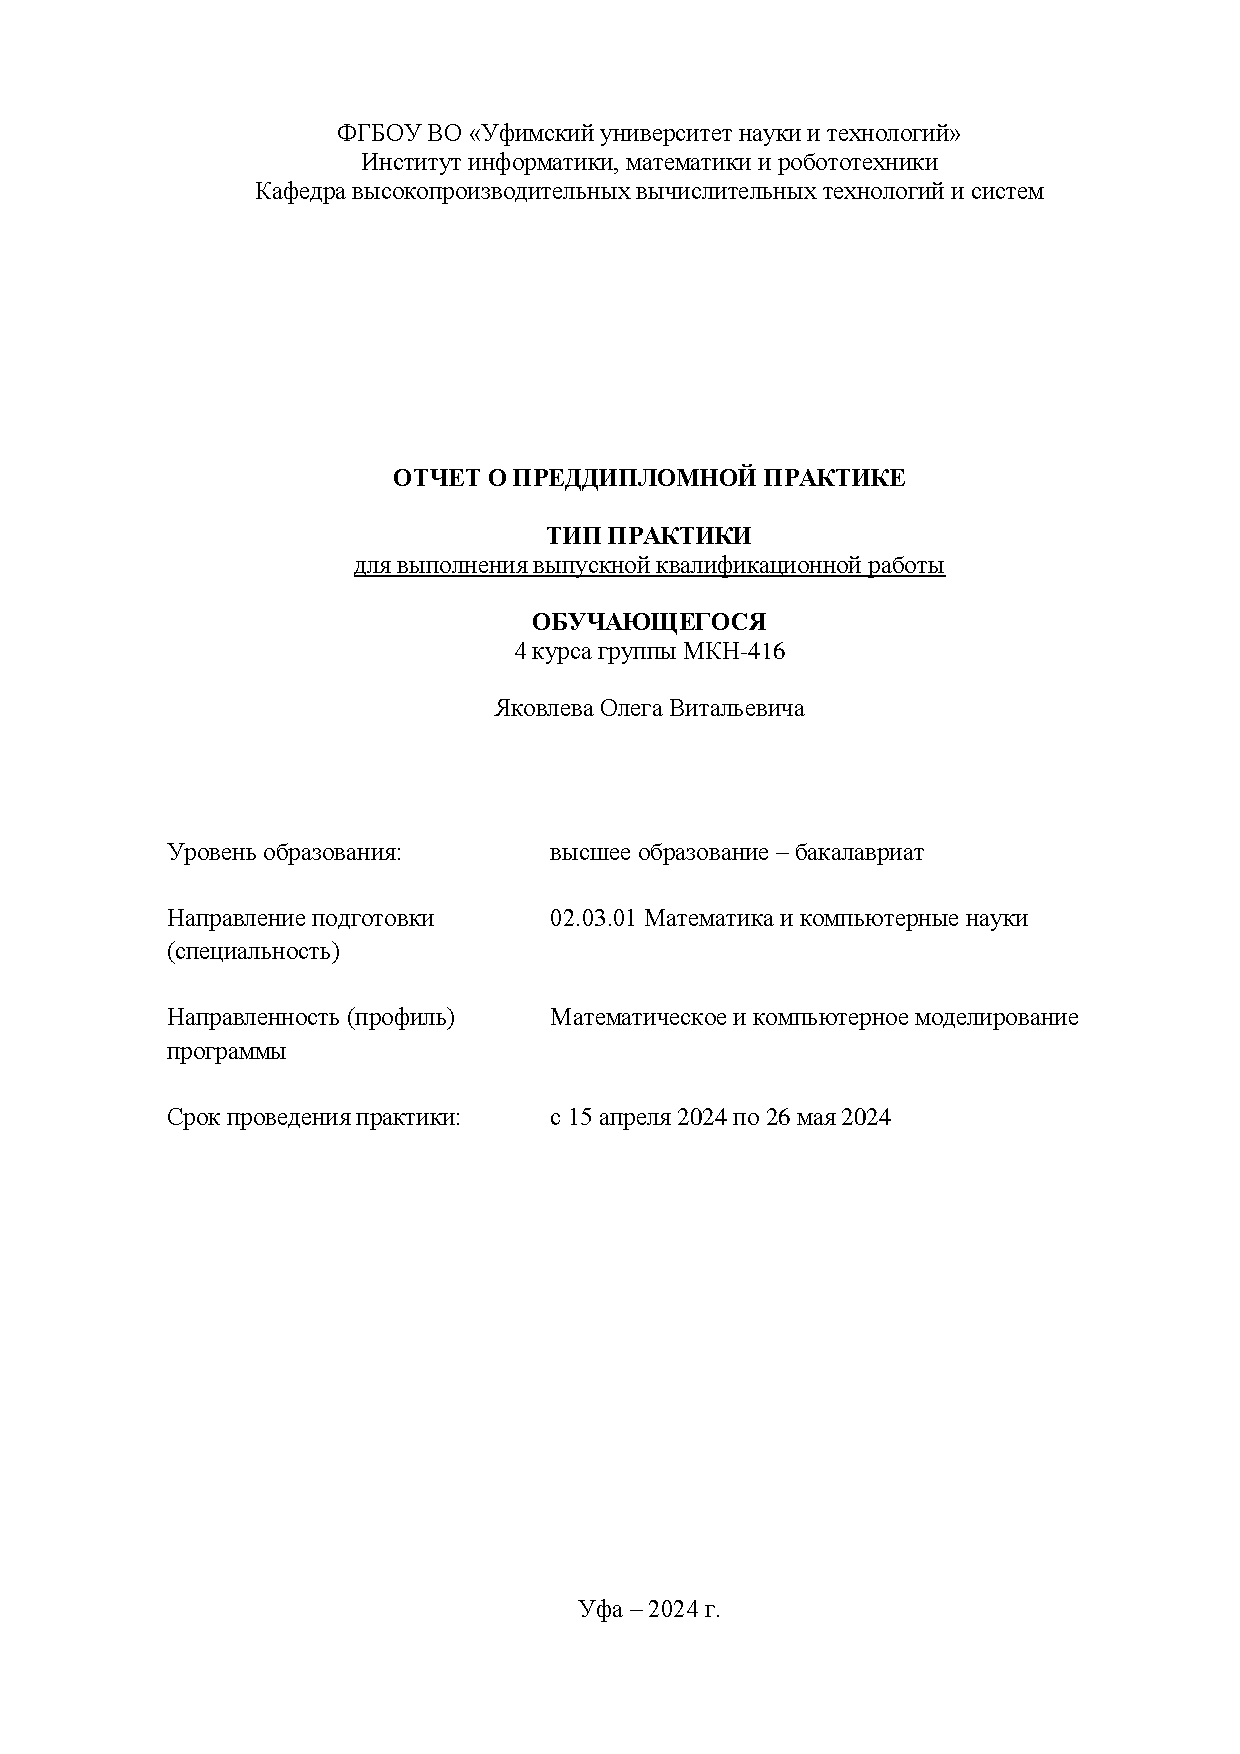
\includepdf[pages=1-9]{cover_pract.pdf}
	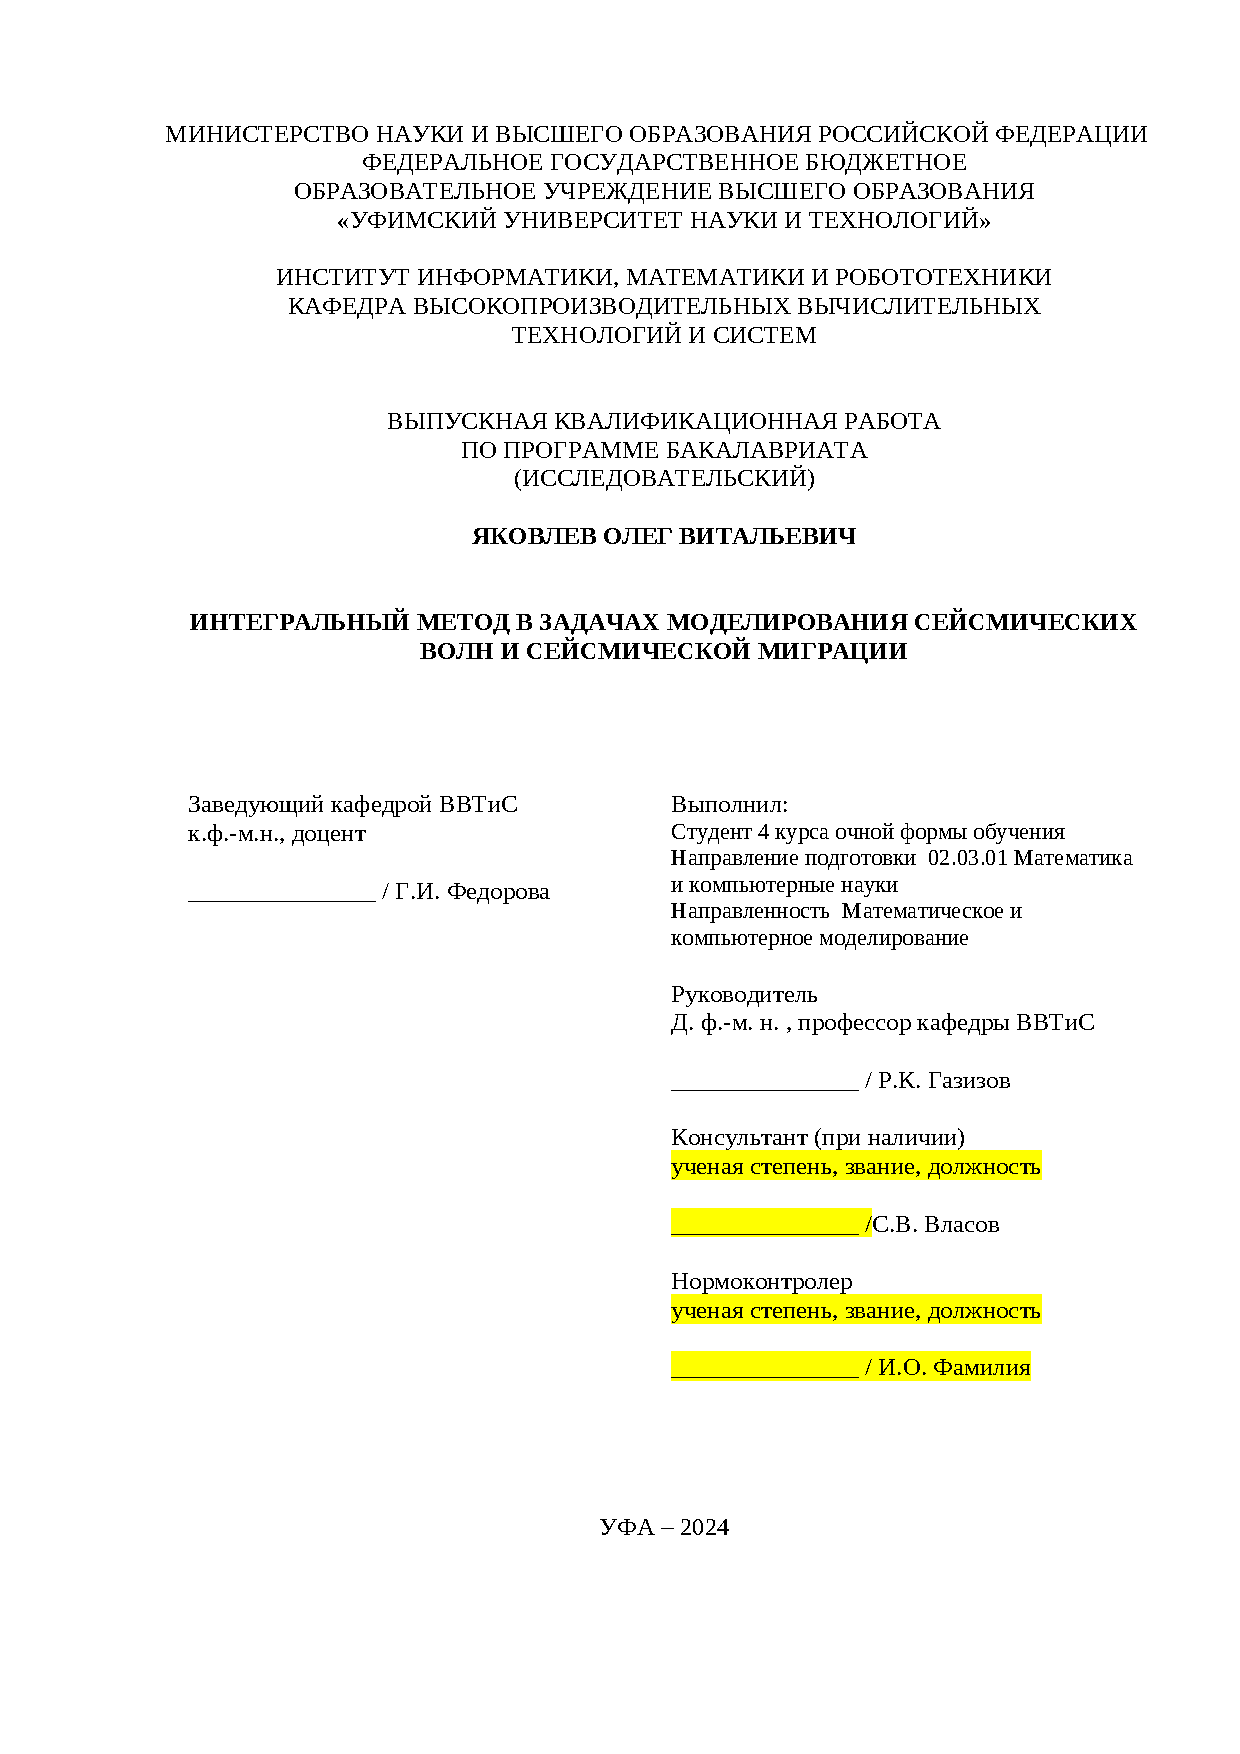
\includepdf[pages=1]{cover_diplom.pdf}
	\section*{Реферат}
	% annotation.tex
	Пояснительная записка \printtotal
	
	\keywords{сейсморазведка, сейсмическое моделирование, миграция, волновое поле, геологоразведка, интеграл Кирхгофа}.
	
	
	В данной работе рассматриваются методы сейсмического моделирования и миграции, которые являются важными инструментами в геологоразведке для определения структуры и состава грунта. Основное внимание уделяется изучению быстрых методов решения прямых и обратных задач сейсморазведки, что необходимо для повышения эффективности и точности разведки нефтегазовых месторождений.
	
	Целью данной работы является разработка численных алгоритмов интегральных методов решения задач сейсмического моделирования и миграции. 
	
	Работа включает теоретическое обоснование и численное моделирование волновых полей, а также демонстрацию применения полученных решений на примерах различных геологических сред. Рассматриваются методы нахождения сейсмических изображений среды по значениям поля на поверхности наблюдения, что позволяет получать точные данные о структуре и свойствах залежей.
	
	Достижения в области сейсмического моделирования и миграции, представленные в данной работе, обеспечивают более надежную интерпретацию сейсмических данных и способствуют развитию методов геофизического исследования.
	
	\newpage 	
	\tableofcontents
	\newpage
	\section*{Введение} 
	\addcontentsline{toc}{section}{Введение}
	
	Проведение геологоразведочных мероприятий позволяет определять структуру
	и состав грунта, что, в свою очередь, позволяет обнаруживать новые
	месторождения полезных ископаемых, а также делать заключения о
	целесообразности разработки того или иного месторождения.
	Одним из наиболее используемых, эффективных и надёжных методов,
	применяемых в геологоразведке, является сейсморазведка, совмещающая в себе
	относительно невысокую стоимость и высокую точность получаемых данных.  
	В ходе обработки данных, полученных в результате сейсмической разведки, 
	возникает необходимость решения прямой и обратной механической задач.
	
	Актуальность применения быстрых методов решения прямых и обратных задач сейсмической разведки обусловлена необходимостью постоянного совершенствования методов геофизического исследования и повышения эффективности разведки нефтегазовых месторождений. Сейсмическое моделирование и миграция являются неотъемлемыми компонентами процесса интерпретации сейсмических данных и предоставляют ценную информацию о структуре и свойствах залежей. В свете постоянно меняющихся условий в нефтегазовой промышленности, эти методы становятся все более важными для обеспечения точности и достоверности геологической информации.
	
	Определения некоторых терминов, использующихся в данной работе:
	\begin{itemize}
		\item Сейсморазведка –- это один из геофизических методов, который преследует задачу
		получения изображения геологической среды с помощью дистанционных методов. 
		
		\item Прямая задача сейсморазведки (сейсмическое моделирование) –- это поиск того, как будет выглядеть 
		искомое физическое поле при заданных параметрах среды. При решении прямой задачи 
		задается известная модель среды с определёнными параметрами и решается задача
		моделирование – на выходе получается сейсмограмма.
		
		\item Обратная задача сейсморазведки (сейсмическая миграция) заключается в определении сейсмического изображения среды по
		наблюдаемому волновому полю (сейсмограммам). Эта задача решается неоднозначно,
		поскольку для одного и того же поля можно получить сразу несколько моделей среды.
		
		\item Сейсмическое изображение среды --  значения поля 	отражённых и дифрагированных волн непосредственно в момент их образования на отражающих границах и локальных неоднородностях	разреза \cite{timoshin}.
		
		\item Сейсмограмма -- это совокупность значений поля отражённых волн, зарегистрированных на земной поверхности.   
	\end{itemize}

	
	Целью данной работы является разработка численных алгоритмов интегральных методов решения задач сейсмического моделирования и миграции. 
	
	Для достижения поставленной цели необходимо решить следующие задачи:
	\begin{enumerate}
		\item Вывести формулу решения задачи сейсмического моделирования в интегральном виде.
		\item Вывести формулу решения задачи сейсмической миграции.
		\item Выполнить программную реализацию алгоритмов интегрального метода решения задач моделирования и миграции.
		\item Провести серию вычислительных экспериментов для решения задачи на конкретном наборе данных.
	\end{enumerate}

	
	\newpage
	\section{Моделирование} 
	\subsection{Постановка задачи сейсмического моделирования} 

	Рассмотрим задачу нахождения значения скалярного волнового поля на поверхности
	наблюдения.
	Допустим задана поверхность, ограничивающая некоторую область пространства
	$D=[0,X]\times [0,Y]\times [0,Z]$.
	Область пространства $D$ разделена на слои $D_1$ и $D_2$ границей $B$, с постоянной
	скоростью звука $c_1$ и $c_2$ соответственно.
	На поверхности наблюдения находятся точечный источник колебаний $S$, который возбуждает
	акустическую волну, являющуюся решением уравнения
	\begin{equation}
		\frac{\partial^2 P}{\partial x^2} + \frac{\partial^2 P}{\partial y^2} +
		\frac{\partial^2 P}{\partial z^2} - \frac{1}{c^2} \frac{\partial^2 P}{\partial
			t^2} = -F(x,y,z,t).
		\label{eq:wav}	
	\end{equation} 
	Модель среды изображена на рисунке \ref{fig:mig}.
	
	\begin{figure}[h]
		
		\centering
		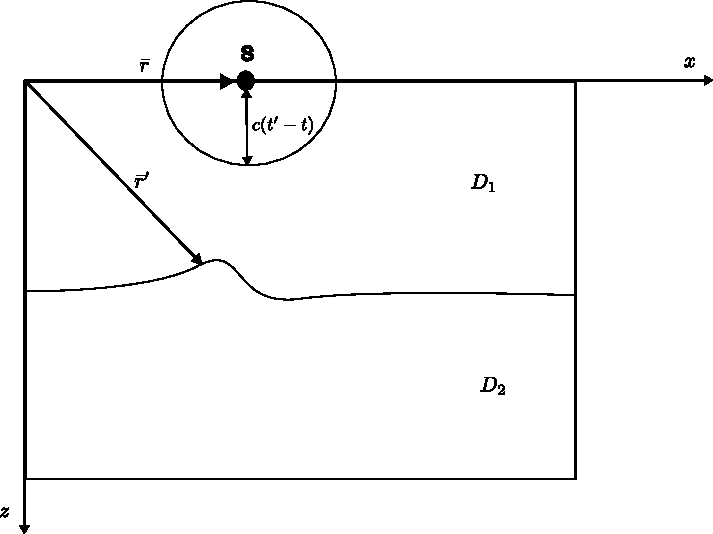
\includegraphics[width=0.9\textwidth]{migration_fig.pdf}
		
		\caption{Модель среды}
		\label{fig:mig}
	\end{figure}
	% DONE RK Сколько источников рассматривается, один или несколько?
	Необходимо по данным характеристикам источника найти значение отражённого волнового поля
	на поверхности наблюдения $z=0$.
	

	%TODO поправить обозначения с соотвествии с рисунком

	%%%%%%%%%%%%%%%%%%%%%%%%%%%%%%%%%%%
	\subsection{Функция Грина} 
		Решение задачи моделирования можно получить при помощи решения
	дифференциального волнового уравнения  \eqref{eq:wav}.

	% DONE RK Функция Дирака не описывает источник колебаний, а только один импульс.
	Рассмотрим импульс мгновенного точечного источника колебаний в трёхмерном пространстве.
	Тогда правая часть уравнения \eqref{eq:wav} будет иметь вид \cite{zhdanov1988}
	\begin{equation}
		F(x,y,z,t) = \delta(t-t_0)\delta(x-x_0)\delta(y-y_0)\delta(z-z_0),
		\label{eq:ptsrc}
	\end{equation}
	Где $\delta(x)$ -- это дельта-функция Дирака.
	\begin{equation}
		\delta(x)=\begin{cases}
			\infty,&x=0,\\
			0,&x\neq 0.
		\end{cases}
		\label{eq:deltadef}
	\end{equation}	
	Решением уравнения \eqref{eq:wav} с правой частью \eqref{eq:ptsrc} является функция
	Грина для волнового уравнения в трёхмерном пространстве.
	
	Пусть источник колебаний находится в начале координат и время импульса $t' = 0$. 
	
	Так как правая часть уравнения равна 0 везде, кроме точки $O(0,0,0)$ в начальный момент времени, поэтому 
	$G$ удовлетворяет уравнению \eqref{eq:uwav} всюду, кроме начала координат
	\begin{equation}
		\frac{\partial^2 G}{\partial x^2} + \frac{\partial^2 G}{\partial y^2} +
		\frac{\partial^2 G}{\partial z^2} - \frac{1}{c^2} \frac{\partial^2 G}{\partial
			t^2} = 0.
		\label{eq:uwav}
	\end{equation}
	Учитывая сферическую симметрию функции Грина, перейдём в уравнении \eqref{eq:uwav} к сферической системе координат
	\begin{equation}
		\frac{1}{r^2}\frac{\partial}{\partial r}\left( r^2 \frac{\partial G}{\partial r} \right)- \frac{1}{c^2} \frac{\partial^2 G}{\partial
			t^2} = 0.
		\label{eq:uswav}
	\end{equation}

	Воспользовавшись равенством $\frac{1}{r}\frac{\partial}{\partial r}\left(r^2\frac{\partial G}{\partial r}\right) = \frac{\partial^2}{\partial r^2}\left(rG\right)$ преобразуем уравнение \eqref{eq:uswav}:
	\begin{equation}
		\frac{\partial^2}{\partial r^2}\left( r  G\right)- \frac{1}{c^2} \frac{\partial^2 }{\partial
			t^2}\left(r G\right) = 0.
		\label{eq:uswav2}
	\end{equation}
	Таким образом мы смогли свести уравнение к одномерному волновому уравнению относительно $F(r,t) = rG$. При помощи замены переменных $\xi = t - \frac{r}{c}$, $\eta = t+\frac{r}{c}$ к простому виду:
	\begin{equation}
		\frac{\partial^2}{\partial \xi \partial \eta} F = 0.
		\label{eq:canonwav}
	\end{equation}
	Интегрируя уравнение \eqref{eq:canonwav}, выразим значение функции Грина из решения дифференциального уравнения:
	\begin{equation}
		G(x,y,z,t) = \frac{1}{r}f\left(t-\frac{r}{c}\right) + \frac{1}{r} g\left(t+\frac{r}{c}\right),
		\label{eq:canonsol}
	\end{equation}
где $r = \sqrt{x^2+y^2+z^2}$.

Первое слагаемое выражения \eqref{eq:canonsol} описывает сферическую волну, которая распространяется от начала координат в бесконечность, а второе слагаемое -- сферическую волну из бесконечности к началу координат. Поскольку, по условиям задачи, источником колебания является единственный источник, то функцию $g$ примем равной нулю.  Чтобы найти функцию  $f$  подставим решение \eqref{eq:canonsol} в уравнение \eqref{eq:wav}. 
\begin{equation}
	\Delta \left[ \frac{1}{r}f\left(t-\frac{r}{c}\right) \right] - \frac{1}{c^2} \frac{\partial^2 }{\partial
		t^2}\left[ \frac{1}{r}f\left(t-\frac{r}{c}\right) \right]  = - \delta(t)\delta(x)\delta(y)\delta(z).
		\label{eq:fwav}
\end{equation}
	%DONE RK Откуда следует это равенство?
Для дальнейшего вывода покажем справедливость следующего равенства \cite{morse}:
	\begin{equation}
		\Delta\left(\frac{1}{r}\right) = -4\pi \delta(x)\delta(y)\delta(z).
		\label{eq:del1r}
	\end{equation}
Проинтегрируем обе части равенства по сфере $E$ с центром в начале координат и радиусом $\varepsilon \to 0$.
\begin{equation}
	\iiint_E \Delta\left(\frac{1}{r}\right) \, dE = -4\pi \iiint_E \delta(x)\delta(y)\delta(z) \, dE.
\end{equation}
По теореме Остроградского-Гаусса можно представить правую часть равенства как интеграл по поверхности сферы $E$.
\begin{equation}
	\iint_{\partial E} \gradop \left(\frac{1}{r}\right) \, dE = -4\pi.
\end{equation}
Так как подынтегральное выражение не зависит от выбора точки на поверхности шара, то предыдущее выражение можно представить в следующей форме:
\begin{equation}
	 \left.\diff{}{r}\left(\frac{1}{r}\right)\right|_{r=\varepsilon} \cdot 4\pi \varepsilon^2 = -4\pi,
\end{equation}	
откуда следует тождество.

Используя равенство \eqref{eq:del1r}, можно привести уравнение \eqref{eq:fwav}
к виду 
\begin{equation}
	-4\pi f(t) \delta(x) \delta(y) \delta(z)  = \delta(x) \delta(y) \delta(z) \delta(t),
\label{eq:fdel}	
\end{equation}
откуда можно выразить значение функции Грина:
\begin{equation}
	G(x,y,z,t) = -\frac{1}{4\pi r} \delta \left(t - \frac{r}{c}\right),
\label{eq:green3d0}	
\end{equation}  
где $r = \sqrt{x^2+y^2+z^2}$.

При выводе формулы \eqref{eq:green3d0} использовалось предположение,  что источник находится в начале координат  и посылает импульс в момент времени $t' = 0$. При переходе к произвольному положению источника 
формула для функции Грина имеет вид
\begin{equation}
	G(\bar{r}',t'|\bar{r}_0,t_0)= \frac{1}{4\pi|\bar{r}'-\bar{r}_0|}
	\delta\left(t'-t_0-\frac{|\bar{r}'-\bar{r}_0|}{c}\right).
\label{eq:green3d}
\end{equation}

	Такая функция Грина называется запаздывающей функцией Грина, так как эффект,
	наблюдаемый в точке $\bar{r}'$ в более поздний момент времени $t'$ вызывается
	возмущением,
	которое произошло в точке $\bar{r}$ в более ранний момент времени $t$.

	
	Для волнового уравнения с произвольной правой частью $F(x,y,z,t)$ можно
	записать формулу представления решения 
	в аналитическом виде при помощи функции Грина, введя вектор $\bar{r} = (x,y,z)$ \cite{vladimirov}:
	
	% TODO RK
	
	
	\begin{equation}
		P(\bar{r}',t')=\iiint\limits_{D_1} \int\limits_{0}^{+\infty}
		F(\bar{r},t) G(\bar{r}' - \bar{r},t'- t)\,dt\,dv.
		\label{eq:wavfgconv}
	\end{equation}
	
	Покажем, что выражение \eqref{eq:wavfgconv} является решением уравнения \eqref{eq:wav} с произвольной правой частью.
	Представим выражение \eqref{eq:wavfgconv} в виде свёртки функций по пространству и времени $P = F*G$. В силу линейности  и теоремы о дифференцировании свёртки функцию $F$ можно вынести из дифференциального оператора.
	Тогда правую часть волнового уравнения записать как 
	\begin{equation}
		\Delta [F*G] -\frac{1}{c^2} \diff[2]{}{t} [F*G] = F*\left[\Delta G -\frac{1}{c^2} \diff[2]{}{t} 
		G\right].
	\end{equation}
	По определению функция Грина является решением волнового уравнения с трёхмерной дельта-функцией в правой части, следовательно
	\begin{equation*}
		F*\left[\Delta G -\frac{1}{c^2} \diff[2]{}{t} G\right] = -F * \delta.
	\end{equation*}
	По свойству дельта-функции 
	\begin{equation}
		-\iiint\limits_{D_1} \int\limits_{-\infty}^{+\infty}
		F(r_0,t_0) \delta({r} - {r}_0,t- t_0)\,dt_0\,dv_0' = -F(x,y,z,t),
	\end{equation}
	что совпадает с исходной правой частью волнового уравнения   \eqref{eq:wav}.
	%DONE ссылка на литру
	
% DONE Связь излучаемого и отраженного волнового поля через коэффициент отражения

% Кирхгоф пока что не нужен
% да блин не нужен тут Борн. Тут сослаться надо на книжку и  сказать, что \lambda = (с1-с2)/(c1+c2)

	
	\subsection{Формула Кирхгофа}
	Для вычисления значения отражённого волнового поля на поверхности наблюдения необходимо 
	рассмотреть как связано значение поля на отражающей границе и значения поля в других точках области, которую ограничивает эта поверхность.   
	% DONE ссылку на будущее уравнение убрать
	Рассмотрим  некоторую ограниченную область пространства $D$, в пределах которой задано скалярное волновое поле, удовлетворяющее следующему уравнению:
	
	\begin{equation}
		\diff[2]{P}{x}  + \diff[2]{P}{y} +
		\diff[2]{P}{z}  - \frac{1}{c^2} \frac{\partial^2 P}{\partial
			t^2} = 0.
		\label{eq:uwav2}
	\end{equation}
	
	 Положим, что граница $S$ области $D$ является кусочно-гладкой. Так как область $D$ ограничена и имеет кусочно-гладкую границу, тогда является справедливым по
	теореме Остроградского-Гаусса:
	\begin{equation}
		\iiint\limits_D \divop F \, dv = \iint\limits_S F \cdot n \, ds.
		\label{eq:vgauss}
	\end{equation}
	Для любых гладких функций $u$ и $v$ справедливо соотношение 
	\begin{equation}
		\divop (u \gradop v) = u\Delta v + \gradop u \cdot \gradop v.
		\label{eq:divgrad1}
	\end{equation}
	Симметрично можно записать:
	\begin{equation}
		\divop (v \gradop u) = v\Delta u + \gradop v \cdot \gradop u.
		\label{eq:divgrad2}
	\end{equation}
	Путём вычитания из уравнения \eqref{eq:divgrad1} уравнения \eqref{eq:divgrad2} получим равенство:
	\begin{equation}
		\divop (u \gradop v - v \gradop u)  = u\Delta v - v \Delta u.
		\label{eq:divgraddiff}
	\end{equation}
	Пусть векторы $r = (x,y,z) \in S$ и $r' = (x',y',z') \in D$ -- это радиус-векторы точек на поверхности $S$ и области $D$ соответственно.
	Положим 
	% DONE RK Надо пояснить, каким уравнениям удовлетворяют P и G.
	\begin{align}
		u(x,y,z,t) =& P(x,y,z,t),\label{eq:subsu}\\
		v(x,y,z,t) = &G(x',y',z',t'|x,y,z,t),\label{eq:subsv}
	\end{align}
	где волновое поле $P$ удовлетворяет уравнению \eqref{eq:uwav2}, 
	а функция Грина $G$ удовлетворяет равенству 
	\begin{equation}
		\diff[2]{G}{x}  + \diff[2]{G}{y} +
		\diff[2]{G}{z}  - \frac{1}{c^2} \frac{\partial^2 G}{\partial
			t^2} = \delta(x-x')\delta(y-y')\delta(z-z')\delta(t-t'),
		\label{eq:wavgdel}
	\end{equation}
	тогда из \eqref{eq:uwav2} и \eqref{eq:wavgdel} соответственно можно выразить 
	% DONE  Ввести вектора r и r'
	% DONE ввести обозначения для случаев, где функция без аргументов
\begin{align}
	% DONE RK Откуда это уравнение?
	\Delta u =& \frac{1}{c^2} \diff[2]{P}{t},\label{eq:subsdu}\\
	\Delta v = &\delta (r' - r) \delta(t' - t) + \frac{1}{c^2} \diff [2]{G(r' -r,t'-t)}{t},\label{eq:subsdv}
\end{align}
где $r=(x,y,z)$. Для краткости обозначим
	\begin{align}
		P =& P(r,t) \\
		G =& G(r',t'|r,t)
	\end{align}
	Проинтегрируем уравнение \eqref{eq:divgraddiff} по времени
	\begin{equation}
		\divop \int\limits_{-\infty}^{+\infty} [P \gradop G - G \gradop P ]\, dt=  P\delta(r-r') +\frac{1}{c^2}\int\limits_{-\infty}^{+\infty}\left[P\diff[2]{G}{t} - G \diff[2]{P}{t}\right]\,dt.
		\label{eq:ugauss}
	\end{equation}
	Интегрированием по частям можно показать, что 
	$$
	\int\limits_{-\infty}^{+\infty}\left[P\diff[2]{G}{t} - G \diff[2]{P}{t}\right]\,dt = 0.
	$$
	Введём обозначение 
	\begin{equation}
			F(x,y,z,t') = \int\limits_{-\infty}^{+\infty} [P \gradop G - G \gradop P ]\, dt,
		\label{eq:kirf}
	\end{equation}
	тогда из уравнений \eqref{eq:ugauss} и \eqref{eq:vgauss} следует
	\begin{equation}
		\iiint\limits_D P\delta(r-r') \, dv = \iint\limits_S F \cdot n \, ds,
	\end{equation}
	где из обозначения \eqref{eq:kirf} следует
	\begin{equation}
		F\cdot n =  \int\limits_{-\infty}^{+\infty} 
		[G(r',t'|r,t)\gradop P(r,t) \cdot n
		- P(r,t)\gradop G(r',t'|r,t) \cdot n] \,dt.
	\end{equation}
Таким образом, получаем соотношение:
	% DONE не физично подставить все до конца раздела
	%TODO На бесконечной области ?
	
	%TODO RK 1. Формула требует пояснения, необходимо дополнить вывод.
	%TODO RK 2. Посмотрите вывод формулы Кирхгофа в классических курсах по УМФ: Тихонов, Самарский; Байков, Жибер.
	\begin{equation}
		P(r',t') = \iint\limits_{\partial D} \int\limits_{-\infty}^{+\infty} 
	[G(r',t'|r,t)\partial_n P(r,t) 
	- P(r,t)\partial_n G(r',t'|r,t)] \,dt\,ds.
	\label{eq:kir}
	\end{equation}
	
	%Для определения в точке $r'$ решения $P(r',t')$ уравнения \ref{eq:wav} введём локальное время $t^* = t - t' + \frac{|r'-r|}{c}$. \cite{samarskii}
Перейдём к сферической системе координат
$$
	u(r,\varphi,\theta,t) = P(r\cos \varphi \cos \theta ,r\sin \varphi \cos \theta,r \sin \theta,t).
$$
$$
	U(r,\varphi,\theta,t) = u(r,\varphi,\theta,t^*).
$$
 Тогда оператор Лапласа будет иметь вид:
\begin{equation}
	\Delta u={\frac{\partial^{2}u}{\partial r^{2}}}+{\frac{2}{r}}{\frac{\partial u}{\partial r}}+{\frac{1}{r^{2}\sin\theta}}{\frac{\partial}{\partial\theta}}\left(\sin\theta{\frac{\partial u}{\partial\theta}}\right)+{\frac{1}{r^{2}\sin^{2}\theta}}{\frac{\partial^{2}u}{\partial\varphi^{2}}}
\end{equation}
Выразим производные функции $u$ через производные $U$:
\begin{gather}
	u_{r}=U_{r^{*}}+{\frac{1}{a}}\,U_{t^{*}}, \\
	u_{r r}=U_{r^{*}r^*}+{\frac{2}{a}}\,U_{r^{*}t}+{\frac{1}{a^{2}}}\,U_{t^{*}t},\\
	u_\theta = U_\theta \\
	u_\varphi = U_\varphi \\
	u_t = U_{t^*} \\
	u_{\theta\theta} = U_{\theta\theta} \\
	u_{\varphi\varphi} = U_{\varphi\varphi} \\
	u_{tt} = U_{t^*t^*} 
\end{gather}
Уравнение \ref{eq:wav} переходит в 
\begin{equation}
	\Delta U=-\frac{2}{a r^{*}}\frac{\partial}{\partial r^{*}}\,(r^{*}U_{t^{*}})-F\,(r^{*},\,\theta^{*},\,t^{*}).
\end{equation}
Рассматривая уравнение как уравнение Лапласа с параметром $t^*$ воспользуемся формулой Грина \cite{samarskii}:
\begin{equation}
	4\pi U\left(M_{0},\,0\right)=\iint_S\left[\frac{1}{r^{\ast}}\,\frac{\partial U}{\partial n}-U\,\frac{\partial}{\partial n}\left(\frac{1}{r^{\ast}}\right)\right]dS + \iiint_T \frac{2}{c r^{*2}} \diff{}{r^*} \left(r^*\diff{U}{t^*}\right) d\tau +
	\iiint_T \frac{F}{r^*} d\tau
\end{equation}
Обозначим $$I = \iiint_T \frac{2}{cr^{*2}} \diff{}{r^*} \left(r^*\diff{U}{t^*}\right) d\tau.$$
Так как $r^*=0$ является сингулярной точкой, вычислим предел
\begin{equation}
	I = \lim\limits_{\varepsilon\to 0} \iiint_{T \setminus T_\varepsilon} \frac{2}{cr^{*2}} \diff{}{r^*} \left(r^*\diff{U}{t^*}\right) d\tau,
\end{equation}
где $T_\varepsilon$ -- шар радиуса $\varepsilon$. Подставим якобиан сферической сисетмы координат
\begin{equation}
	d\tau = r^{*2} \sin \theta\, dr\,d\theta \, d\varphi,
\end{equation}
\begin{equation}
	I = \lim\limits_{\varepsilon\to 0} \iiint_{T \setminus T_\varepsilon} \frac{2}{c} \diff{}{r^*} \left(r^*\diff{U}{t^*}\right) \sin \theta\, dr\,d\theta \, d\varphi.
\end{equation}
Проинтегрируем по $r$
\begin{equation}
	I =  \iint_{S} \frac{2}{cr^*} \left(\diff{U}{t^*}\right) \cos(n,r) dS - \lim\limits_{\varepsilon\to 0} \iint_{S_\varepsilon} \frac{2}{cr^*} \left(\diff{U}{t^*}\right) \cos(n,r) dS
\end{equation}
Так как радиус $T_\varepsilon$ стремится к нулю, то и предел в предыдущем выражении также равен нулю.
Таким образом получаем интегральную формулу 
\begin{equation}
	u\left(M_{0},t_{0}\right)=\frac{1}{4\pi}\iint_{S}^{}\left\{\frac{1}{r}\left[\frac{\partial u}{\partial n}\right]-\left[u\right]\frac{\partial}{\partial n}\left(\frac{1}{r}\right)+\frac{1}{a r}\left[\frac{\partial u}{\partial t}\right]\frac{d r}{d n}\right\}d S_{M}+\iiint_T\frac{[f]}{r}\,d\tau
	\label{eq:kirsam}
\end{equation}


	
	Это соотношение носит название интегральной формулы Кирхгофа.
	Интегральная
	формула Кирхгофа показывает, как можно восстановить волновое поле внутри области,
	ограниченной некоторой поверхностью, по значениям этого поля (и его нормальной
	производной) на границе области.
	
	Подставим в формулу \eqref{eq:kir} функцию Грина \eqref{eq:green3d} для однородного трёхмерного пространства:
	\begin{multline}
		P\left(r',t'\right)=\frac{1}{4\pi}\iint_{\partial D}^{}\left\{\frac{1}{|r'-r|}\left[\frac{\partial P}{\partial n}\right]-\left[P\right]\frac{\partial}{\partial n}\left(\frac{1}{|r'-r|}\right)+ \right. \\ 
		+\left. \frac{1}{c |r'-r|}\left[\frac{\partial P}{\partial t}\right]\frac{d r'}{d n}\right\}d D,
		\label{eq:kirg0}
	\end{multline}
		где квадратные скобки обозначают значения функций для $t=t'-\frac{|r'-r|}{c}$.
	
	\begin{figure}[h]
		\centering
		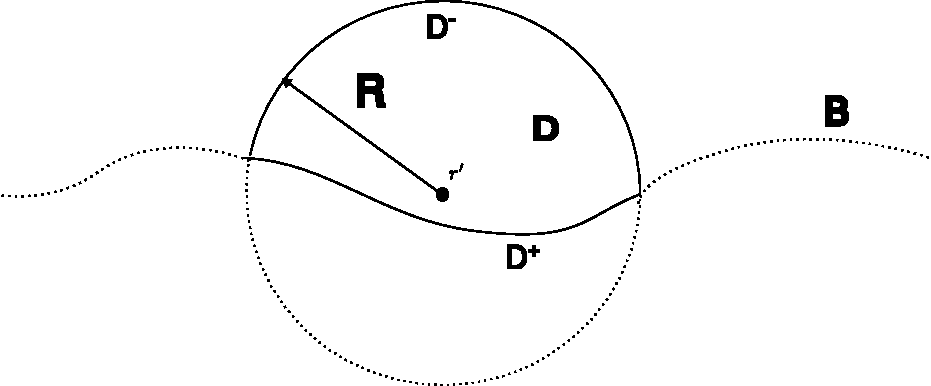
\includegraphics[width=0.7\textwidth]{kir_inf.pdf}
		\caption{}
		\label{fig:kir_inf}
	\end{figure}
	
	Пусть область $D$ (изображена на рисунке \ref{fig:kir_inf}) ограничена сверху бесконечной горизонтальной границей $B$, а снизу -- сферой с центром в точке $r'$ радиуса $R$. Обозначим область поверхности $B$ внутри сферы как $D^+$, а границу сферы выше поверхности $B$ как $D^-$. Для границы области $D$ справедлива формула Кирхгофа \eqref{eq:kirg0}.
	Обозначим 
	\begin{gather*}
		I^+=\frac{1}{4\pi}\iint_{D^+}^{}\left\{\frac{1}{|r'-r|}\left[\frac{\partial P}{\partial n}\right]-\left[P\right]\frac{\partial}{\partial n}\left(\frac{1}{|r'-r|}\right)+\frac{1}{c |r'-r|}\left[\frac{\partial P}{\partial t}\right]\frac{d r'}{d n}\right\}d D, \\
		I^-=\frac{1}{4\pi}\iint_{D^-}^{}\left\{\frac{1}{R}\left[\frac{\partial P}{\partial n}\right]-\left[P\right]\frac{\partial}{\partial n}\left(\frac{1}{R}\right)+\frac{1}{c R}\left[\frac{\partial P}{\partial t}\right]\frac{d r'}{d n}\right\}d D,	
	\end{gather*}
	Тогда интеграл Кирхгофа \eqref{eq:kirg0} можно представить в виде суммы 
	\begin{equation*}
		P(r',t') = I^+ +I^-.
	\end{equation*}
	
	При устремлении $R \to \infty$ выражение $I^-$ стремится к нулю. Следовательно, для полупространства выше поверхности $B$ можно записать:
	\begin{equation}
		P\left(r',t'\right)=\frac{1}{4\pi}\iint_{B}^{}\left\{\frac{1}{|r'-r|}\left[\frac{\partial P}{\partial n}\right]-\left[P\right]\frac{\partial}{\partial n}\left(\frac{1}{|r'-r|}\right)+\frac{1}{c |r'-r|}\left[\frac{\partial P}{\partial t}\right]\frac{d r'}{d n}\right\}d D.
	\end{equation}
	
	%TODO ???????????????????????????????????????????????????????????????????????????????????????????
	Далее, необходимо получить выражение для волнового поля, отражённого от отражающей границы.
	Волновое поле, созданное точечным источником, удовлетворяет неоднородному уравнению
	\begin{equation}
		\frac{\partial^2 P_0}{\partial x^2} + \frac{\partial^2 P_0}{\partial y^2} +
		\frac{\partial^2 P_0}{\partial z^2} - \frac{1}{c^2} \frac{\partial^2 P_0}{\partial
			t^2} = -f(t)\delta(x-x_0)\delta(y-y_0)\delta(z-z_0).
	\end{equation}
	Решение этого уравнения можно представить в интегральном виде, используя формулу \eqref{eq:wavfgconv}:
	\begin{equation}
		P_0(r,t) = \frac{f(t-\frac{|r-r_0|}{c})}{4\pi|r-r_0|}.
	\end{equation}
	Отражённое волновое поле связано с падающим волновым полем через коэффициент отражения: 
	\begin{equation}
		P_1(r,t) = \Lambda(r) \cdot P_0(r,t)
	\end{equation}
	\begin{equation}
		\diff{}{n}P_1(r,t) = -\Lambda(r) \cdot  \diff{}{n} P_0(r,t)
	\end{equation}
	Продолжим отражённое  волновое поле наверх при помощи интегральной формулы Кирхгофа \eqref{eq:kir}:
	\begin{equation}
		P\left(r_0',t'\right)=\frac{1}{4\pi}\iint_{B}^{}\left\{\frac{1}{|r_0'-r|}\left[\frac{\partial P_1}{\partial n}\right]-\left[P_1\right]\frac{\partial}{\partial n}\left(\frac{1}{|r_0'-r|}\right)+\frac{1}{c r}\left[\frac{\partial P_1}{\partial t}\right]\frac{d r_0'}{d n}\right\}d B,
		\label{eq:kirp0}
	\end{equation}
	где квадратные скобки обозначают значения функций для $t=t'-\frac{|r'-r|}{c}$, $r\in B$,  $r_0'$ принадлежит плоскости $z=0$.
	Так как величины $\frac{1}{|r_0'-r|}$ и $\frac{1}{|r-r_0|}$ меняются достаточно медленно   по сравнению с  $f$ \cite{buchen}, то при дифференцировании можно принять их за постоянные:
	\begin{equation}
		P\left(r',t'\right)=\frac{1}{4\pi}\iint_{B}^{}\left\{\frac{1}{|r'-r|}\left[\frac{\partial P_1}{\partial n}\right]+\frac{1}{c |r'-r|}\left[\frac{\partial P_1}{\partial t}\right]\frac{d (r'-r)}{d n}\right\}d B,
	\end{equation}
	\begin{equation}
		\frac{\partial P_1}{\partial n}=\Lambda(r)\frac{f'(t-\frac{|r-r_0|}{c})}{4\pi|r-r_0|c} \cdot \cos (n,r-r_0) ,
	\end{equation}
	\begin{equation}
		\diff{P_1}{t}=\Lambda(r)\frac{f'(t-\frac{|r-r_0|}{c})}{4\pi|r-r_0|} ,
	\end{equation}
	\begin{equation}
		\frac{d r_0'}{d n}= \cos (n,r_0'-r).
	\end{equation}

	

	%DONE RK Вывод и графическое пояснение.
	\begin{equation}
		P(r',t') = \iint\limits_{B} \left[\Lambda(r) \frac{f'\left(t'-\frac{|r'-r|+|r-r_0|}{c}\right) }{16\pi^2c|r'-r||r-r_0|} (\cos \psi_1 + \cos \psi_2) \right] \,dB
		\label{eq:modapx}
	\end{equation}
где $\psi_1$ -- угол между нормалью к поверхности $B$ и вектором $r_0'-r$,
$\psi_2$ -- угол между нормалью к поверхности $B$ и вектором $r-r_0$. 

\begin{figure}[h]
	\centering
	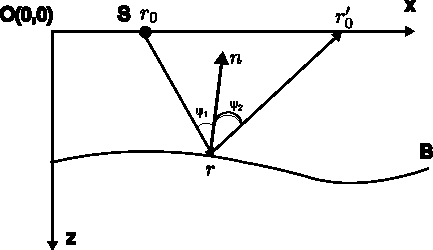
\includegraphics[width=0.7\textwidth]{model_fig.pdf}
	\caption{}
	\label{fig:model}
\end{figure}
%TODO рисунок
Обозначим суммарное время от источника колебаний в точке $r_0$ до точки на отражающей поверхности $r$ и от $r$ до заданной точке на поверхности наблюдения $r_0'$ за $$\tau(r_0',r) =\frac{|r_0'-r|+|r-r_0|}{c},$$ а коэффициент, зависящий от $r$ и $r'$ -- за 
$$
	W(r',x,y,z) = - \frac{\cos \psi_1 + \cos \psi_2}{8\pi c|r'-r||r-r_0|}.
$$ 



Можно представить полученное выражение в виде интеграла, представляющего решение задачи сейсмического моделирования: \cite{pokr}:
% DONE RK Как выводится (1.3.17)?
\begin{equation}
	P(r_0',t') = \frac{1}{2\pi} \iint_{z=B(x,y)} W(r_0',x,y,z) f'[t-\tau(r_0',r)] dB,
	\label{eq:modpokr}
\end{equation}
где $W(r_0',x,z)$ -- весовая функция, зависящая от функции Грина и угла падения волны на отражатель.
	\subsection{Уравнение Гельмгольца и коэффициент отражения}
	Для дальнейших рассуждений будет удобно перейти от временной области в частотную. Представим поле $P(r,t)$ как суперпозицию полей в частотной области $p(r,\omega)$:
	\begin{equation}
		P(r,t) =  \int_{-\infty}^{\infty} p(r,\omega) e^{i\omega t}\, d\omega.
	\end{equation}
	Применим преобразование Фурье к волновому уравнению \eqref{eq:wav}:
	\begin{equation}
		\int_{-\infty}^{\infty} \left[ \nabla^2 P(r,t) + \frac{1}{c^2}\diff[2]{P(r,t)}{t}\right] e^{-i\omega t} \, dt = - \int_{-\infty}^{\infty}   F(r,t) e^{-i\omega t} \, dt.
	\end{equation}
	По свойствам преобразования Фурье производная по времени переходит в частотной области в умножение на коэффициент 
	$i\omega$. В результате получаем уравнение, называемое {\it уравнением Гельмгольца}:
	\begin{equation}
		\nabla^2 p(r,\omega) + \frac{\omega^2}{c^2}p(r,\omega) = - f(r,\omega).
		\label{eq:helmholtz}
	\end{equation}

	Рассмотрим отражение звуковой волны в плоскости $xz$ от плоской границы раздела сред $z=0$. Волну созданную точечным источником колебаний на большом удалении можно приблизительно считать плоской. 

	Плоской волной называется решение волнового уравнения \eqref{eq:uwav2} вида $$P(\xi) := P\left(\frac{n_xx+n_yy+n_zz}{c}-t\right),$$ где $n(n_x,n_y,n_z)$ -- нормаль к фронту волны.
	При помощи преобразования Фурье выразим плоскую как интеграл по гармоническим колебаниям частоты $\omega$:
	\begin{equation}
		P(\xi) = \int \limits_{-\infty}^{\infty} p(r,\omega) e^{i\omega \xi}\, d\xi.
	\end{equation}

	Пусть на плоскость падает плоская гармоническая волна $e^{i\frac{\omega}{c_1}(x\sin \theta - z\cos \theta)}$.
	Обозначим амплитуду падающей волны за единицу, амплитуду отражённой волны за $V$, а амплитуду преломлённой волны за $W$.
	Тогда выражения для падающей, отражённой и преломлённой волн можно записать в виде \cite{brehovskih} 
	%DONE RK Откуда следуют эти формулы?
	\begin{gather}
		p_0(r,\omega) = e^{i\frac{\omega}{c_1}(x\sin \theta - z\cos \theta)},\label{eq:reflp0}\\ 
		p_1(r,\omega) = \Lambda e^{i\frac{\omega}{c_1}(x\sin \theta + z\cos \theta)},\label{eq:reflp1}\\
		p_2(r,\omega) = W e^{i\frac{\omega}{c_2}(x\sin \theta_2 - z\cos \theta_2)}\label{eq:reflp2}.
	\end{gather}
	где $\theta$ и $\theta_2$ обозначают углы падения и преломления соответственно. Волны \eqref{eq:reflp1} и \eqref{eq:reflp2} удовлетворяют уравнению 
	\begin{equation}
		\nabla^2 p(r,\omega) + \frac{\omega^2}{c_1^2}p(r,\omega) = - f(r,\omega),
	\end{equation}
	а  \eqref{eq:reflp2} удовлетворяет уравнению
	\begin{equation}
		\nabla^2 p(r,\omega) + \frac{\omega^2}{c_2^2}p(r,\omega) = 0.
	\end{equation}
	
	При отражении акустической волны от границы на поверхности раздела должны быть равны давления и нормальные скорости в обеих средах \cite{landavshic}.
	
	\begin{gather}
		z=0,\label{eq:rc1}\\
		\lim_{z_0\to 0+0} p(x,y,z_0,\omega) = \lim_{z_0\to 0-0} p(x,y,z_0,\omega), \label{eq:rc2}\\
		\lim_{z_0\to 0+0} \diff{p(x,y,z_0,\omega)}{z} = \lim_{z_0\to 0-0} \diff{p(x,y,z_0,\omega)}{z}.\label{eq:rc3}
	\end{gather}
	Полное поле из условия \eqref{eq:rc2} можно выразить как 
	%TODO RK 
	\begin{equation}
		p(r,\omega) = \begin{cases}
			p_0(r,\omega)+p_1(r,\omega) \quad r\in D_1, \\
			p_2(r,\omega) \quad r \in D_2.
		\end{cases}
	\end{equation}
	
	Таким образом, на границе раздела выполняются условия \eqref{eq:rc1} и \eqref{eq:rc2}, следовательно выполняется равенство
	\begin{equation}
		(1+\Lambda)= W e^{i\frac{\omega}{c_2}x\sin \theta_2  - ix\frac{\omega}{c_1}\sin \theta}
	\end{equation}
	Так как левая часть последнего равенства не зависит от $x$, то значит  коэффициент перед  $x$ в правой части равен нулю:
	\begin{equation}
		\frac{\sin \theta_2}{c_2} = \frac{\sin \theta}{c_1}.
	\label{eq:snell}
	\end{equation}
	Последнее равенство называется законом Снелля.
	
	Для гармонической волны в однородной среде плотностью $\rho$ колебательная скорость в звуковой волне записывается \cite{landavshic}:
	\begin{equation}
		v = \frac{\gradop p}{i\omega \rho}.
	\end{equation}
	
	Введём понятие акустического импеданса:
	\begin{equation}
		Z = -\frac{p}{v_z}.
	\end{equation}
	Вычислим импеданс в области $D_1$:
	\begin{equation}
		Z_1 = -\frac{i\omega \rho_1 c_1 (e^{i\frac{\omega}{c_1}(x\sin \theta - z\cos \theta)}+\Lambda e^{i\frac{\omega}{c_1}(x\sin \theta + z\cos \theta)})}{i\omega(-e^{i\frac{\omega}{c_1}(x\sin \theta - z\cos \theta)}+\Lambda e^{i\frac{\omega}{c_1}(x\sin \theta + z\cos \theta)}) \cos \theta },
	\end{equation}
	\begin{equation}
		Z_1 = -\frac{ \rho_1 c_1 (e^{i\frac{\omega}{c_1}(- z\cos \theta)}+\Lambda e^{i\frac{\omega}{c_1}( z\cos \theta)})}{(-e^{i\frac{\omega}{c_1}( - z\cos \theta)}+\Lambda e^{i\frac{\omega}{c_1}(z\cos \theta)}) \cos \theta }.
		\label{eq:impz1}
	\end{equation} 
	Аналогично для области $D_2$:
	\begin{equation}
		Z_2 = \frac{i\omega c_2 \rho_2 W e^{i\frac{\omega}{c_2}(x\sin \theta_2 - z\cos \theta_2)}}{i\omega W e^{i\frac{\omega}{c_2}(x\sin \theta_2 - z\cos \theta_2)}\cos \theta_2},
	\end{equation}
	\begin{equation}
		Z_2 = \frac{ c_2 \rho_2 }{ \cos \theta_2}.
	\end{equation}
	Из условий \eqref{eq:rc2} и \eqref{eq:rc3} можно сделать вывод, что импеданс на поверхности раздела сред также является непрерывной величиной.
	\begin{equation}
		\left.Z_1\right|_{z=0} = \left. Z_2 \right|_{z=0}
	\end{equation}
	\begin{equation}
		\frac{1+\Lambda }{1-\Lambda } = \frac{c_2 \rho_2 \cos \theta }{c_1 \rho_1 \cos \theta_2 }
	\end{equation}
	Обозначим импеданс падающей волны за $Z = \frac{c_1\rho_1}{\cos \theta}$:
	\begin{equation}
		\frac{1+\Lambda }{1-\Lambda } = \frac{Z_2 }{Z}.
	\end{equation}
	Выражая $\Lambda $ из предыдущего выражения получим
	\begin{equation}
		\Lambda =\frac{Z_2-Z}{Z_2+Z}.
		\label{eq:lambdaZ}
	\end{equation}
	Подставим в выражение \eqref{eq:lambdaZ} значения для импедансов $Z_2$ и $Z$:
	\begin{equation}
		\Lambda = \frac{c_2 \rho_2 \cos \theta - c_1 \rho_1 \cos \theta_2}{c_2 \rho_2 \cos \theta + c_1 \rho_1 \cos \theta_2}.
		\label{eq:lambda}
	\end{equation}
	% DONE ссылку на нормальную литературу.
	Таким образом, можно записать выражение для продолжения отражённого волнового поля \eqref{eq:modapx}:
	\begin{equation}
		P(r',t') = \iint\limits_{B} \left[ \frac{c_2 \rho_2 \cos \theta - c_1 \rho_1 \cos \theta_2}{c_2 \rho_2 \cos \theta + c_1 \rho_1 \cos \theta_2} \cdot \frac{f'\left(t'-\frac{|r'-r|+|r-r_0|}{c_1}\right) }{16\pi^2c_1|r'-r||r-r_0|} (\cos \psi_1 + \cos \psi_2) \right] \,dB,
	\end{equation}
	где угол падения $\theta=\psi_1$.
	Для вычисления значения косинусов углов $\psi_1$, $\psi_2$ можно воспользоваться скалярным произведением:
	\begin{gather}
		\cos \psi_2=\frac{(r'-r)\cdot n }{|r'-r|}, \\
		\cos \psi_1 = \frac{(r-r_0)\cdot n }{|r-r_0|}.  \label{eq:cosincident}
	\end{gather}
	Косинус угла преломления $\theta_2$ можно выразить из закона Снелля \eqref{eq:snell}:
	\begin{equation}
		\cos \theta_2 =  \sqrt{1-\frac{c_2^2}{c_1^2}(1-\cos^2 \psi_1)}.
	\end{equation}


	
	
 %%  Смотри born_approx.tex 

	
	%TODO: зачем приближение Борна нужно?
	%TODO ссылки на литру про приближение Борна
	\subsection{Приближение Борна}
	В задаче сейсмического моделирования часто возникает необходимость нахождения волнового поля, отражённого от границ ограниченной области (называемой областью неоднородности), где скорость распространения звуковой волны отличается от скорости в окружающем пространстве. Чтобы учесть все области отражающей поверхности, на которые падает волна, созданная источником, воспользуемся приближением Борна для отражённой волны.\cite{zhdanov2007}
	
	Рассмотрим задачу нахождения отраженного волнового поля $P_1(r',t)$ от эллиптической границы области неоднородности $D_1$ со скоростью звука  $c_2$ в окружающем пространстве $D$ со скоростью звука $c_1$ в заданном поле $P_0(r,t)$. 
	
	
	Представим скорость распространения волны в виде
	\begin{equation}
		\frac{1}{c^2(r)} = \frac{1+a(r)}{c_1^2},
	\end{equation}
	где $a(r)$ -- это функция, не равная нулю внутри области неоднородности поля.
	  
	Обозначим значение, обратное по величине скорости волны, как медленность 
	\begin{gather*}
		s = \frac{1}{c}, \\
		s_1 = \frac{1}{c_1}, \\
		s_2 = \frac{1}{c_2}.
	\end{gather*}
	Таким образом функция $a(r)$ является квадратом нормированной аномальной медленности:
	$$
	a(r) = \frac{s^2 - s_1^2}{s_1^2} = \frac{\Delta s^2}{s_1^2}
	$$
	Падающее волновое поле удовлетворяет волновому уравнению в области $D_1$ при $t>0$:
	\begin{equation}
		\nabla^2 P_0 - \frac{1}{c_1^2}\diff[2]{P_0}{t} = 0.
		\label{eq:wavp0}
	\end{equation}
	Преломлённое волновое поле также является решением волнового уравнения, но в области $D_2$ с другой скоростью звука:
	\begin{equation}
		\nabla^2 P_2 - \frac{1}{c_2^2}\diff[2]{P_2}{t} = 0.
		\label{eq:wavp2}
	\end{equation}
	Из условия \eqref{eq:rc2} непрерывности значения  волнового поля на границе однородной области можно переписать уравнение \eqref{eq:wavp2} в виде
	\begin{equation}
		\nabla^2 P_0 + \nabla^2 P_1 - \frac{1}{c_2^2}\diff[2]{P_0}{t} - \frac{1}{c_2^2}\diff[2]{P_1}{t}  = 0.
		\label{eq:wavp01sum}
	\end{equation}
	Подставим в выражение $\nabla^2 P_0$ из уравнения \eqref{eq:wavp0}, и
	тогда отражённое волновое поле будет удовлетворять уравнению \cite{bleistein2012mathematical}
	\begin{equation}
		\nabla^2 P_1 - \frac{1}{c_2^2}\diff[2]{P_1}{t}  = - \frac{1}{c_1^2}\diff[2]{P_0}{t} + \frac{1}{c_2^2}\diff[2]{P_0}{t}.
	\end{equation}
	Так как отражённая волна распространяется в области $D_1$, то она удовлетворяет следующему неоднородному волновому уравнению:
	\begin{equation}
		\nabla^2 P_1 - \frac{1}{c_1^2}\diff[2]{P_1}{t}  = \left(\frac{1}{c_2^2} - \frac{1}{c_1^2}\right)\left(\diff[2]{P_0}{t} + \diff[2]{P_1}{t}\right).
		\label{eq:wavp1inh}
	\end{equation}
	Используя введённые ранее обозначения, перепишем уравнение \eqref{eq:wavp1inh} следующим образом:
	\begin{equation}
		\nabla^2 P_1 - \frac{1}{c_1^2}\diff[2]{P_1}{t}  = \Delta s^2 \cdot \diff[2]{P_2}{t}.
	\end{equation}
	Следовательно, решение этого неоднородного дифференциального уравнения можно выразить через функцию Грина:
	\begin{equation}
		P_1(r',t')   = \iiint\limits_{D_1} \int\limits_{-\infty}^{\infty} \Delta s^2 \cdot \left(\diff[2]{P_0(r,t)}{t}+\diff[2]{P_1(r,t)}{t}\right) G(r',t'|r,t)\, dt \, dv.
	\end{equation}
	Приближение Борновского типа состоит в том, чтобы положить отражённое поле под знаком интеграла равным нулю:
	\begin{equation}
		P_1(r',t')   = \iiint\limits_{D_1} \int\limits_{-\infty}^{\infty} \Delta s^2 \cdot 	\diff[2]{P_0(r,t)}{t} G(r',t'|r,t)\, dt \, dv.
	\end{equation}
	
	Рассмотрим вычисление отражённого поля на примере неоднородности в форме эллипсоида. Пусть эллиптическая граница области неоднородности задана уравнением:
	\begin{equation}
		\frac{x^2}{A^2} + \frac{y^2}{B^2} + \frac{z^2}{C^2} = 1
	\end{equation}
	
	Перейдём в обобщённую полярную систему координат:
	\begin{align*}
		x &= A \rho \cos \phi \cos \theta, \\
		y &= B \rho \sin \phi \cos \theta, \\
		z &= C \rho \sin \theta. 
	\end{align*}
	Таким образом значение поля, отражённого от эллипсоида, можно вычислить при помощи следующей формулы:
	\begin{equation}
		P_1(r_0',t') = \frac{\Delta s^2}{4\pi} \int_{0}^{2\pi} \int_{-\frac{\pi}{2}}^{\frac{\pi}{2}} \int_{0}^{1} \frac{ABC \rho^2 \cos \theta}{|r_0'-r|} \diff[2]{}{t}P_0(r,t' - \frac{|r_0'-r|}{c_2}) \,d\rho \, d\phi \, d \theta.
		\label{eq:bornellipse}
	\end{equation}
	
	
	\section{Миграция}
	\subsection{Постановка задачи сейсмической миграции}
	%TODO FIXME: постановка задачи
	
	Пусть возбуждение и регистрация колебаний происходит на плоской горизонтальной поверхности. Пусть
	существует некоторая неизвестная граница, которую мы хотим определить, при этом распределение скорости в пространстве
	между свободной поверхностью и границей считается известным. 
	
	Такую задачу можно свести к задаче нахождения обращённого продолжения $W(r',t')$ ($t' = T-t$) поля $P(r,t)$ ($r=(x,y,0),t\in[0,T]$), зарегистрированного на поверхности $z=0$ \cite{petrashen}. 
	Под обращённым продолжением понимается решение уравнения
	\begin{equation}
		\Delta W + \frac{1}{c^2} \diff[2]{W}{t} = 0
	\end{equation}
	в области $z<0$ с нулевыми начальными условиями и граничным условием
	\begin{gather*}
		\left.W\right|_{t'=0} = 0, \\
		\left.\diff{W}{t'}\right|_{t'=0} = 0, \\
		 \left.W\right|_{z=0} = P(r,t).
	\end{gather*}
	
	Рассмотрим гипотетическую волну, двигающуюся вверх к поверхности наблюдения с направлением, которое в определённый момент времени (например, при $t = 0$) совпадает с одной из отражающих границ. Далее, очевидно, что волна будет распространяться вдоль тех же лучей, что и реальное отражённое поле <<нулевого удаления>>, которое было зарегистрировано совмещёнными источниками и приёмниками, для времени $t>0$. Это связано с тем, что лучи первичной и отражённой волн должны совпадать, если положения источников и приёмников совпадают. Это возможно только в том случае, если соответствующая траектория луча нормальна к отражающей границе. Таким образом, как и предполагаемая волна, которую мы называем восходящей волной Клербо, и реальное отражённое волновое поле, зарегистрированное совмещёнными источниками и приёмниками, они должны распространяться вдоль одних и тех же лучевых путей. Тем не менее волне Клербо потребуется пятьдесят минут, чтобы достичь определённой точки на поверхности наблюдения, куда придёт реальная отражённая волна, которая должна пройти это расстояние дважды. Тем не менее обе волны достигнут любой точки поверхности наблюдения одновременно, если предположить, что скорость волны Клербо в среде в два раза меньше, чем скорость реальной волны \cite{zhdanov2007}.

	\subsection{Интеграл Рэлея}
	Для восстановления волн, которые распространяются по направлению к поверхности наблюдения, в качестве фундаментального решения нужно использовать функцию, сопряжённую к функции Грина волнового уравнения.
	\begin{equation}
	\widetilde{G}( r,t|r',t')=G(r,-t|r,-t).
	\end{equation}
	В случае постоянной скорости звука, эта функция имеет вид:
	\begin{equation}
	\widetilde{G}(r,t\mid r',t')=\frac{1}{4\pi\left|r-r'\right|}\delta\left(\frac{\left|r-r'\right|}{c}+(t-t')\right).
	\end{equation}
	Для того, чтобы функция соответствовала значениям волнового поля на поверхности наблюдения, необходимо и достаточно, чтобы выполнялось равенство
	\begin{equation}
	\iint_{S}\int_{-\infty}^{\infty}{\widetilde{G}}\left(r'',t^{\prime}|r,t\right){\frac{\partial}{\partial n}}P(r,t)d t\,d s = \iint_{S}\int_{-\infty}^{\infty}P(r,t){\frac{\partial}{\partial n}}{\widetilde{G}}\left(r'',t^{\prime}|r,t\right)\,d t\,d s.
	\end{equation}
	Пусть точки $r'$ и $r''$ расположены симметрично относительно $S$. Тогда справедливы для любой точки $r\in S$
	\begin{align}
		\widetilde{{{G}}}\left({r}^{\prime\prime},t^{\prime}|{r},t\right)~~&=~~\widetilde{G}\left({r}^{\prime},t^{\prime}|{r},t\right), \\
		\frac{\partial}{\partial n}\widetilde G\left({ r}^{\prime\prime},t^{\prime}|{ r},t\right)~&=~-\frac{\partial}{\partial n}\widetilde G\left({ r}^{\prime},t^{\prime}|{ r},t\right).
	\end{align}
	В результате получается тождество для любого ${ r}^{\prime}\in V$.
	\begin{equation}
	\iint_{S}\int_{-\infty}^{\infty}\widetilde{G}\left({r}^{\prime},t^{\prime}|{r},t\right)\frac{\partial}{\partial n}P({r},t)d t\,d s = -\iint_{S}\int_{-\infty}^{\infty}P({ r},t){\frac{\partial}{\partial n}}\widetilde{G}\left({ r}^{\prime},t^{\prime}|{ r},t\right)\,d t\,d s.
	\label{eq:req0}
	\end{equation}
Подставляя соотношение \eqref{eq:req0} в \eqref{eq:kir} можно модифицировать интеграл Кирхгофа в выражение, 
известное как интегральная формула Рэлея:
\begin{equation}
P({ r}^{\prime},t^{\prime})=2\iint_{S}\int_{-\infty}^{\infty}P({ r},t)\frac{\partial}{\partial z}\widetilde{G}\left({ r}^{\prime},t^{\prime}|{ r},t\right)d t d s.
\label{eq:rayleighorig}
\end{equation}
	По принципам восстановления изображения среды на основе миграционного преобразования, необходимо получить изображение отражающих границ путём построения распределения восходящего волнового поля в нижнем полупространстве в момент $t' = 0$. Для среды с постоянной волновой скоростью интеграл Релэя будет иметь вид
	\begin{equation}
		P(r',0) = \frac{1}{2\pi} \iint_S \int_{-\infty}^{\infty} P(r,t) \frac{\partial}{\partial z} 
		\left[ \frac{\delta(2|r'-r|/c -t)}{|r'-r|}\right]\,dt\,ds.
		\label{eq:rayleighsingular}
	\end{equation}
	Соотношение \eqref{eq:rayleighsingular} нельзя использовать для построения практических алгоритмов миграции из-за присутствия сингулярности. Вынося производную за знаки интегрирования и вычисляя свёртку по времени с дельта-функцией, получим следующее выражение\cite{golubev}:
	\begin{equation}
				P(r',0) = \frac{1}{2\pi}\frac{\partial}{\partial z} \iint_S   
		\left[ \frac{P(r,2|r'-r|/c)}{|r'-r|}\right]\,ds
		\label{eq:rayleighgood}
	\end{equation}
	%TODO:  Написать про алгоритм?
	%\begin{comment}
	%TODO постановка задачи и численное решение
	

	\section{Результаты расчётов и анализ результатов}
	В данной работе для расчётов была разработана программа на языке C++, 
	численное нахождение определённых интегралов
	производилось методом прямоугольников. В программе можно задавать максимальное и минимальное количество используемых ячеек памяти.
	
	Рассмотрим область пространства $D = [0,X]\times [0,Y] \times [0,Z]$ в течение отрезка времени $[0,T]$. При дальнейших расчётах для данной задачи, будем полагать 
	$X = 50$, $Y=50$ и $T=1$. Пусть точечный источник колебаний расположен на поверхности наблюдения $z_0=0$ в середине рассматриваемой области: $x_0 = 25$, $y_0 = 25$. Необходимо определить значение отражённого волнового поля на поверхности $z=0$. 
	
	Можем положить, что точечный источник колебаний имеет функцию импульса в виде импульса Рикера:
	\begin{equation}
		f(t) = P_0 \cdot (1-2\pi^2 \nu^2 t^2)\exp(-\pi^2 f^2 t^2).
	\end{equation}
	При дальнейших расчётах используем следующие параметры импульса источника: 
	\begin{align*}
		\nu &=10, \\
		P_0 & = 1.
	\end{align*}
	
	Для вычисления отражённого поля от произвольной границы горизонтально-слоистой среды необходимо найти время распространения волны между точками, расположенными на границах.  Пусть $r_a^n$ обозначает радиус-вектор точки $a$, находящейся на границе номер $n$.
	Обозначим время распространения волны между точками $r_a^n$ и $r_b^m$ на горизонтальных границах $\Delta t (r_a^n,r_b^m)$.
	Так как $\Delta t (r_a^n,r_b^m) = \Delta t (r_b^m,r_a^n)$, положим $n<m$. Тогда время распространения волны между точками на границах можно вычислить при помощи рекуррентной формулы:
	$$
	\Delta t (r_a^n,r_b^m) = \begin{cases}
		\min\limits_{k} \left( \Delta t (r_a^n,r_k^{m-1}) + \frac{|r_b^m-r_k^{m-1}|}{c_{m-1}}\right) & m > n+1, \\
		\frac{|r_b^m-r_a^n|}{c_{m-1}} & m = n+1. \\
	\end{cases}
	$$
	
	Для вычисления значения интеграла в формуле  \eqref{eq:modapx} воспользуемся методом трапеций. 
	Обозначим подынтегральное выражение за $K$:
	\begin{equation}
			K(x,y) = \left[\Lambda(r(x,y,z(x,y)) \frac{f'\left(t'-\Delta t(r_0,r) - \Delta t(r,r_0')\right) }{16\pi^2c|r_0'-r||r-r_0|} (\cos \psi_1 + \cos \psi_2) \right].
	\end{equation}
	Тогда численное значение интеграла можно вычислить при помощи значений подынтегрального выражения на двухмерной сетке 
	\begin{equation}
					P(r',t')=\frac{1}{2} \left(\sum_{i,j=0}^{N-1} K(x_i,y_j) \Delta x \Delta y + \sum_{i,j=1}^{N} K(x_i,y_j) \Delta x \Delta y\right), 
	\end{equation}
	где $N$ -- количество узлов сетки,  $\Delta x = \frac{X}{N}$ -- размер сетки по оси $x$,  $\Delta y = \frac{Y}{N}$ -- размер сетки по оси $y$, 
	%TODO инт 
	
	% FILE: error.tex
	Сравним точность интегрирования методом трапеций и численного интегрирования при помощи квадратуры Гаусса на примере вычисления сейсмограммы нулевого удаления отражённой волны от горизонтальной границы на глубине $H$.
	Для вычисления отражённого волнового поля воспользуемся выражением \eqref{eq:modapx}. Так как вычисляется сейсмограмма нулевого удаления, то положение источника и приёмника сейсмических колебаний совпадают: $r' = r_0$. Тогда формулу  \eqref{eq:modapx} можно упростить:
	\begin{equation}
		P(r_0,t') = \iint\limits_{B} \left[\Lambda(r) \frac{f'\left(t'-\frac{2|r-r_0|}{c}\right) }{16\pi^2c|r-r_0|^2} (2\cos \psi_1 ) \right] \,dB
	\end{equation}
	Параметризуем подынтегральное выражение с помощью $\rho = |r-r_0|$ и перейдём к полярной системе координат:
	\begin{equation}
		P(r_0,t') = \int_0^{2\pi}  \int_H^{\infty} \left[\Lambda(r) \frac{f'\left(t'-\frac{2\rho}{c}\right) }{16\pi^2c\rho^2} (2\cos \psi_1 ) \right] d\rho\,d\theta.
	\end{equation}
	Отражающая плоскость является бесконечной, поэтому значение отражённого поля не зависит от положения источника и приёмника $r_0$ на поверхности $z=0$.
	Так как плоскость горизонтальная, то $\cos \psi_1 = \frac{H}{\rho}$:
	\begin{equation}
		P(t') = H \int_H^{\infty} \left[ \frac{c_2 \rho_2 \cos \theta - c_1 \rho_1 \cos \theta_2}{c_2 \rho_2 \cos \theta + c_1 \rho_1 \cos \theta_2}  \cdot \frac{f'\left(t'-\frac{2\rho}{c}\right) }{4\pi c\rho^3}  \right] d\rho,
	\end{equation}
	где $\cos \theta = \frac{H}{\rho}$,  $\cos \theta_2 = \sqrt{1-\frac{c_2^2 H^2}{c_1^2\rho^2}}$.
	
	\begin{figure}[H]
		\centering
		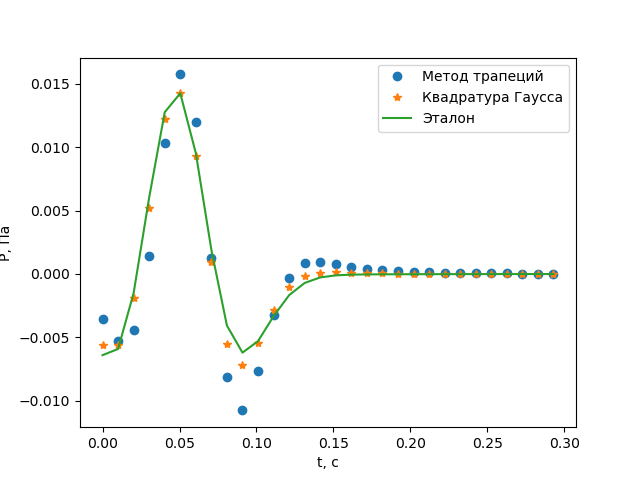
\includegraphics[width=.8\textwidth]{trapgauss.png}
		\caption{}
		\label{fig:trapgauss}
	\end{figure}
	
	На рисунке \ref{fig:trapgauss} изображены графики отражённого поля давления на поверхности, смоделированных с применением различных методов интегрирования. За эталон принимаются данные, использованные в академическом турнире.  Максимальная абсолютная погрешность вычислений с  использованием метода трапеций составляет $\Delta = 0.0046$ Па.
	Максимальная абсолютная погрешность вычислений с  использованием квадратуры  Гаусса составляет $\Delta = 0.0014$ Па.
	Максимальная относительная погрешность вычислений с  использованием метода трапеций составляет $\delta = 32.4\%$ .
	Максимальная относительная погрешность вычислений с  использованием квадратуры  Гаусса составляет $\delta = 10\%$.
	
	
	\subsection{Отражение от плоской горизонтальной границы} \label{sect:horizontal}
	
	Пусть на глубине $h_1 = 2$ расположена плоская горизонтальная граница раздела сред со скоростями звука $C_1$ и $C_2$. 
	Расчёты были выполнены с использованием следующих значений скоростей распространения волны внутри слоёв среды:
\begin{align*}
	C_1 &= 108 \\
	C_2 &= 140 
\end{align*}
	
\begin{figure}[H]
	\centering
	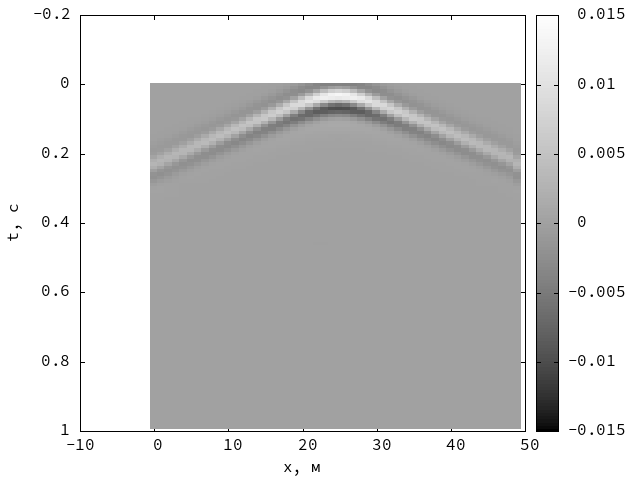
\includegraphics[width=.7\textwidth]{smooth_single_seism.png}
	\caption{Значение отражённого от границы слоёв поля давления на поверхности наблюдения $z = 0$ для различных моментов времени $t\in [0,1]$ в сечении $y=25$.}
	\label{fig:single_hor}
\end{figure}
%    ...
	На рисунке \ref{fig:single_hor} представлена сейсмограмма колебаний, зарегистрированных у поверхности земли. На графике ось $x$ направлена вправо, ось $t$ направлена  вниз.
	Из рисунка видно, что волна, созданная источником колебаний на поверхности земли, отражается от границы раздела однородных слоёв и достигает поверхности земли за время $t_1 = 0.037$ и распространяется по поверхности со скоростью $C_1$. 
	\subsection{Отражение от границ горизонтально-слоистой среды}
	Далее рассмотрим случай трёхслойной и четырёхслойной среды. Пусть верхние слои имеют соответственную толщину $h_1 = 2$, $h_2 = 18$, $h_3 = 24$, а нижний слой занимает оставшееся полупространство. Скорость звука в каждом из слоёв соответственно равна:
	\begin{align*}
		C_1 &= 108,\\
		C_2 &= 140,\\
		C_3 &= 180,\\
		C_4 & = 216.
	\end{align*}
	\begin{figure}[H]
	\begin{subfigure}{.5\textwidth}
		\centering
		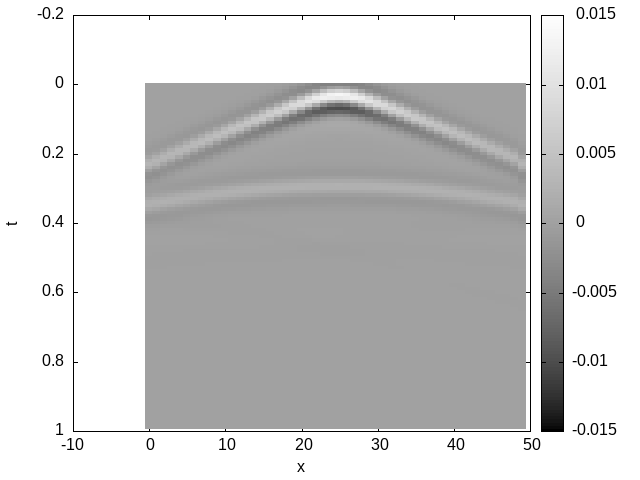
\includegraphics[width=\textwidth]{smooth_double_far_seism.png}
		\caption{Отражение от двух границ слоёв.}
		\label{fig:multi_hor2}
	\end{subfigure}
	\begin{subfigure}{.5\textwidth}
		\centering
		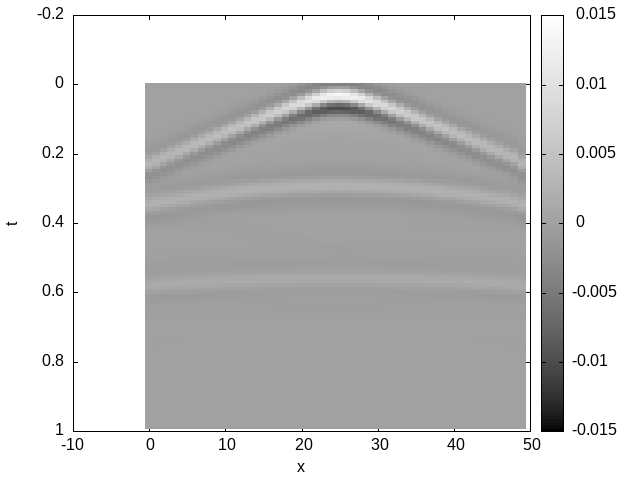
\includegraphics[width=\textwidth]{smooth_triple_far_seism.png}
		\caption{Отражение от трёх границ слоёв.}
		\label{fig:multi_hor3}
	\end{subfigure}
	\caption{Значение поля давления, отражённого от нескольких границ слоёв, на поверхности наблюдения $z = 0$ для различных моментов времени $t\in [0,1]$ в сечении $y=25$.}
	\label{fig:multi_hor}
\end{figure}

	На рисунках \ref{fig:multi_hor2} и \ref{fig:multi_hor3} представлены сейсмограммы колебаний, зарегистрированных у поверхности земли. На графиках ось $x$ направлена вправо, ось $t$ направлена  вниз. 
	
	Из рисунка \ref{fig:multi_hor2} видно, что, помимо волны, отразившейся от первой границы, в момент времени $t_2 = 0.29$ поверхности $z=0$  достигает волна, отразившаяся от второй границы между слоями. Амплитуда второй волны ниже амплитуды первой из-за большей удалённости данной границы от поверхности наблюдения. 
	
	На рисунке \ref{fig:multi_hor3} волна отражённая от третьей границы в момент времени $t_3 = 0.56$.
	
	\subsection{Отражение от плоской наклонной границы}
		
Рассмотрим случай двухслойной среды, когда граница между слоями является наклонная плоскость. Значения скоростей внутри каждого слоя зададим равными 
\begin{align*}
	C_1 &= 72, \\
	C_2 &= 120.
\end{align*}
	Пусть граница между слоями задана уравнением (ось $z$ направлена вниз):
	\begin{equation}
		z = 0.15 x + 0.15 y + 1.
	\end{equation}
	\begin{figure}[H]
		\centering
		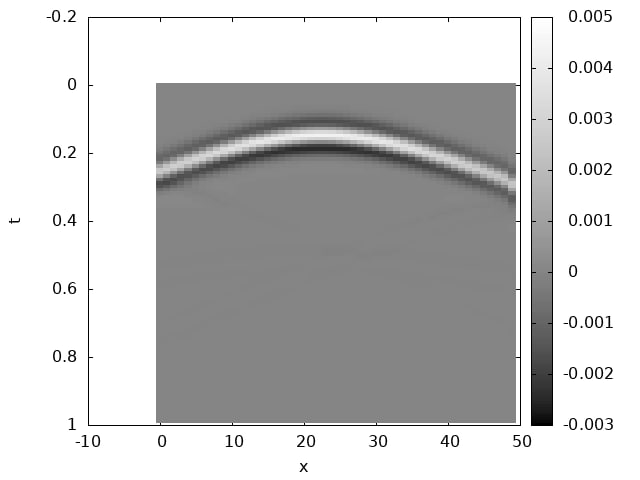
\includegraphics[width=.7\textwidth]{tilted15.png}
		\caption{Значение поля давления, отражённого от наклонной границы, на поверхности наблюдения $z = 0$ для различных моментов времени $t\in [0,1]$ в сечении $y=25$.}
		\label{fig:tilt}
	\end{figure}
	На рисунке \ref{fig:tilt} изображена сейсмограмма волнового поля, отражённого от наклонной плоской границы раздела сред. Волна, порождённая точечным источником, отражается от наклонной плоскости и достигает поверхности наблюдения за время $t_4 = 0.43$. % TODO как волна сместилась?
	
	\subsection{Отражение от сферической неоднородности}

	Рассмотрим случай, когда отражающая граница не является плоской, а представляет собой границу сферы. Пусть задана область неоднородности (изображена на рисунке \ref{fig:spheremod}), границы которой заданы уравнением 
	\begin{equation}
		(x-x_0)^2 + (y-y_0)^2 + (z-z_0)^2 = R^2.
	\end{equation}
	\begin{figure}[h]
		\centering
		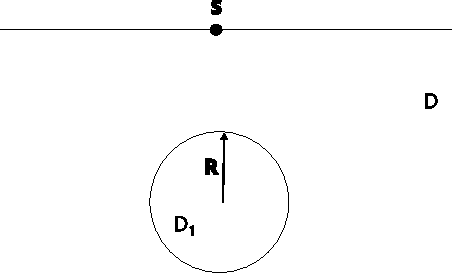
\includegraphics{sphere_mod.pdf}
		\caption{Область сферической неоднородности.}
		\label{fig:spheremod}
	\end{figure}
	
	Центр сферы расположен в точке $x_0 = 25, y_0 = 25,z_0 = 25$.
	Пусть в окружающем пространстве задана скорость звука $C_1 = 72$, а внутри области неоднородности задана скорость распространения волны $C_5 = 8$.
	
	
	\begin{figure}[H]
		\begin{subfigure}{.5\textwidth}
			\centering
			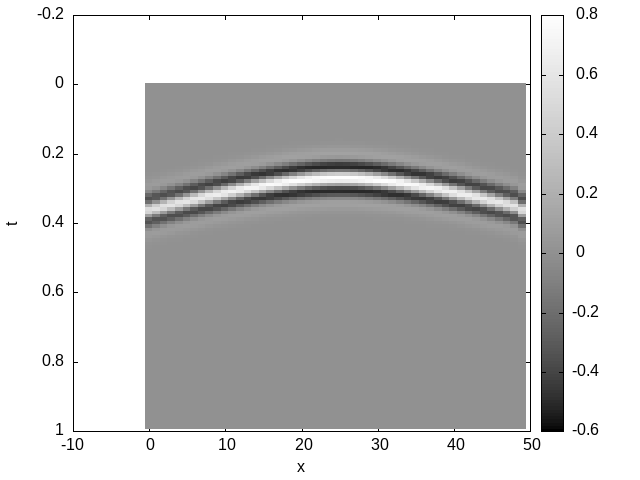
\includegraphics[width=\textwidth]{sphere_3_seism.png}
			\caption{$R=3$.}
			\label{fig:sphere3}
		\end{subfigure}
		\begin{subfigure}{.5\textwidth}
			\centering
			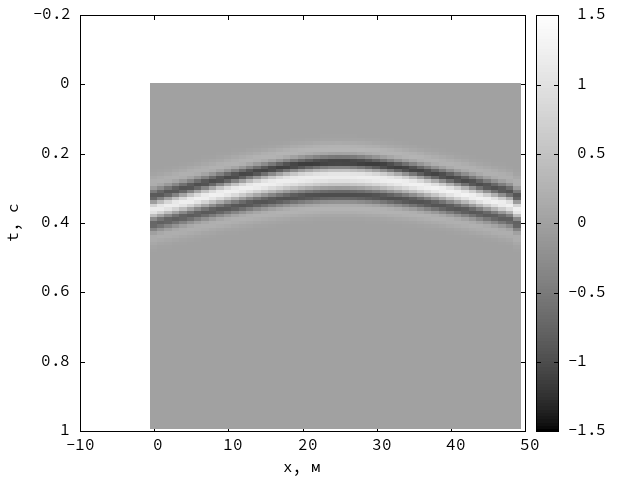
\includegraphics[width=\textwidth]{sphere_5_seism.png}
			\caption{$R=5$.}
			\label{fig:sphere5}
		\end{subfigure}
		\caption{Сейсмограмма волнового поля отражённого от сферической границы с различными радиусами области неоднородности.}
	\end{figure}
	
	На рисунках \ref{fig:sphere3} и \ref{fig:sphere5} изображены сейсмограммы  колебаний, отражённых от сферической границы области неоднородности.
	Волна, созданная источником колебаний на поверхности наблюдения, достигает отражателя и возвращается на поверхность $z=0$ за время $t_5 = 0.35$ при $R=3$ и $t_5=0.35$ при $R=5$.
	При увеличении радиуса области неоднородности  амплитуда и продолжительность увеличивается. 
	  
	
	\begin{comment}
	\subsection{Отражение в горизонтально-слоистой среде с эллиптическим включением}
	Рассмотрим область пространства $D = [0,X]\times [0,Y] \times [0,Z]$ в течение отрезка времени $[0,T]$. Пусть среда разделена на горизонтальные слои с заданной толщиной, в каждом из которых задана скорость распространения звуковой волны (рисунок \ref{fig:layers}). Внутри третьего слоя задана неоднородность в форме эллипсоида: 
	\begin{equation}
		\frac{(x-x_0)^2}{A^2} + \frac{(y-y_0)^2}{B^2} + \frac{(z-z_0)^2}{B^2} = 1.
	\end{equation}
	На поверхности через равные промежутки расположены совмещённые источники и приёмники сейсмических колебаний. Необходимо вычислить значение волнового поля в точках расположения приёмников на поверхности.  
	\begin{figure}[H]
		\centering
		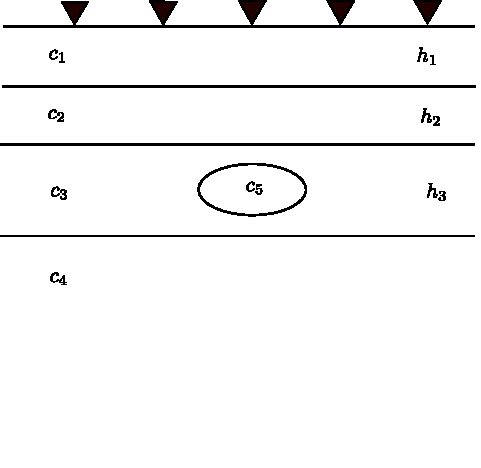
\includegraphics[width=0.5\textwidth]{layers.pdf}
		\caption{Модель слоистой среды с эллиптическим включением.}
		\label{fig:layers}
	\end{figure}
	
	Пусть мощности слоёв и скорости звука в однородных слоях соответственно равны: 
	\begin{gather*}
		h_1 = 200, c_1 = 1800, \\
		h_2=199, c_2 = 3000,\\
		h_3=297, c_3 = 4500,\\
		c_4 = 5400.
	\end{gather*}
	Значения параметров эллиптической неоднородности:
	\begin{gather*}
		x_0 = 2610,\\
		y_0 = 493, \\
		A = 100, \\
		B = 45.
	\end{gather*}
\end{comment}
	\subsection{Сейсмическое изображение горизонтальной плоской границы}
	Теперь рассмотрим задачу нахождения расположения горизонтальной границы по известному значению отражённого волнового поля на поверхности наблюдения $z=0$. Пусть известно волновое поле на поверхности и распределение скоростей в каждом из слоёв. Необходимо определить глубину, на которой находится отражающая граница. 
	
	 В качестве начальных данных используем значения волнового поля и распределения скоростей, рассчитанные ранее в разделе \ref{sect:horizontal}. 
	
	\begin{figure}[H]
		\centering
		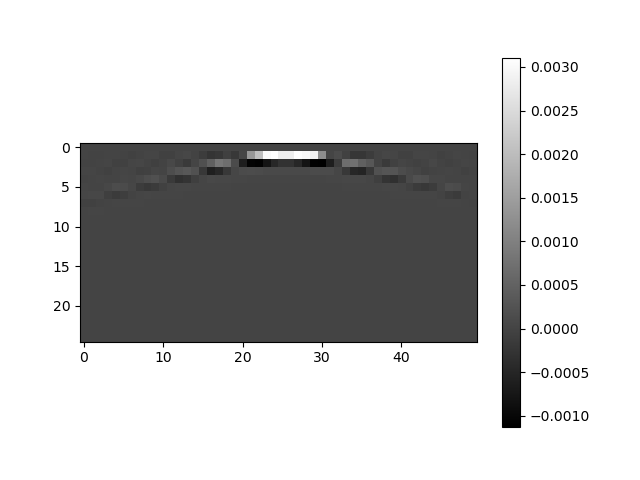
\includegraphics[width=.7\textwidth]{mig_horizontal_single.png}
		\caption{Сейсмическое изображение среды с горизонтальной отражающей границей в сечении $y=25$.}
		\label{fig:mig_hor}
	\end{figure}
	
	На рисунке \ref{fig:mig_hor} показано сейсмическое изображение среды, полученное при помощи преобразования сейсмической миграции. 
	На графике ось $x$ направлена вправо, ось $z$ направлена вниз.
	На изображении видно, что отражённая волна, зарегистрированная на поверхности наблюдения, в момент отражения находилась на глубине $z = 2$.
	
	
	\subsection{Сейсмическое изображение наклонной плоской границы}
	
	Далее, рассмотрим задачу нахождения плоской наклонной по известному значению отражённого волнового поля на поверхности наблюдения $z=0$.
	Пусть известно волновое поле на поверхности и распределение скоростей в каждом из слоёв. Необходимо определить положение наклонной границы в пространстве.
	
	На поверхности наблюдения расположены точечные источники колебаний, совмещённые с сейсмическими приёмниками. 
	Сейсмограмма, полученная при такой конфигурации источников и приёмников, называется сейсмограммой нулевого удаления \cite{timoshin}. 
	\begin{figure}[H]
		\centering
		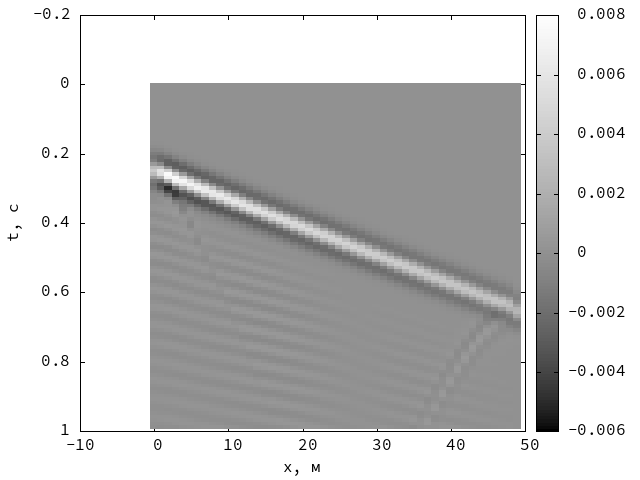
\includegraphics[width=.7\textwidth]{tilt15c36_centr_seism.png}
		\caption{Сейсмограмма нулевого удаления волнового поля, отражённого от наклонной отражающей границы, при совмещённых источниках  в сечении $y=25$.}
		\label{fig:mig_tilt_seism}
	\end{figure}
	Рассчитаем значения отражённого поля на поверхности, при следующих параметрах среды: 
	\begin{align*}
		C_1 &= 36, \\
		C_2 &= 60,
	\end{align*}
	наклонная граница между слоями задана уравнением:
	\begin{equation}
		z=1+0.15 x+0.15 y.
		\label{eq:mig_mod}
	\end{equation}
	На рисунке \ref{fig:mig_tilt_seism} изображена сейсмограмма полученного волнового поля.
	По смоделированным значениям при помощи преобразования миграции можно определить положение отражающей границы между однородными слоями.  
	
	
	\begin{figure}[H]
		\centering
		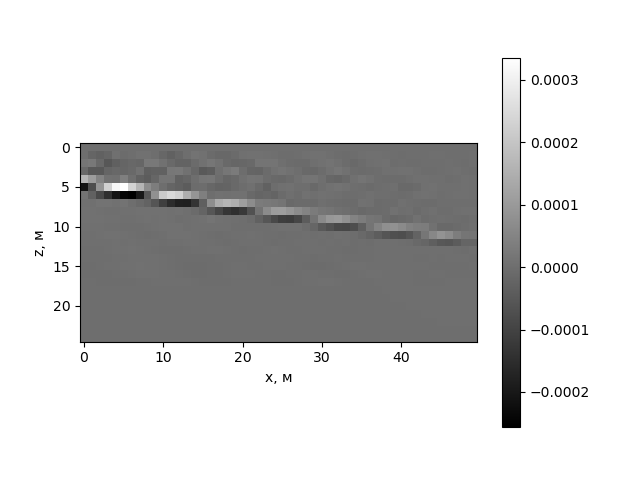
\includegraphics[width=.9\textwidth]{mig_tilted_central_ok.png}
		\caption{Сейсмическое изображение нулевого удаления среды с наклонной отражающей границей в сечении $y=25$.}
		\label{fig:mig_tilt}
	\end{figure}
	На рисунке \ref{fig:mig_tilt} показано сейсмическое изображение среды, полученное при помощи преобразования сейсмической миграции. 
	На графике ось $x$ направлена вправо, ось $z$ направлена вниз. На изображении видно, что волны, порождённые источниками на поверхности наблюдения, отражаются от наклонной плоскости.  По данному сейсмическому изображению можно определить коэффициент наклона плоскости вдоль оси $x$: $$m = \frac{11-5}{45-5}.$$ Значение $m=0.15$ соответствует уравнению \eqref{eq:mig_mod}. 
	
	
	
	\clearpage
	
	
	\section*{Заключение} \addcontentsline{toc}{section}{Заключение}
	В данной работе была построена модель распространения  акустической волны в некоторой области
	 пространства, при помощи записи решения волнового уравнения в интегральной форме и продолжения поля при
	 помощи интеграла Кирхгофа. Была показана связь между амплитудой волны, достигающей границы раздела
	  однородных сред, и амплитудой волны, отражённой от границы раздела сред, при помощи коэффициента
	  отражения.
	
	Была выполнена численная программная реализация модели и продемонстрирована её работоспособность на примерах решения задач моделирования отражённого волнового поля от слоистой среды для случаев: одной горизонтальной границы, нескольких горизонтальных границ, плоской наклонной границы, сферической границы. Выполнено сравнение методов численного интегрирования на примере решения задачи моделирования сейсмограммы нулевого  удаления для поля, отражённого от горизонтальной плоской границы. В ходе сравнения показано, что численное интегрирование при помощи квадратуры Гаусса даёт более точный результат ($ \delta = 10\%$) по сравнению с методом трапеций ($\delta = 32.4\%$).
	
	Далее, была рассмотрена задача нахождения сейсмического изображения среды по значениям поля на поверхности наблюдения. Записано решение задачи обратного продолжения волны, восходящей к поверхности наблюдения. 
	Была выполнена численная программная реализация решения задачи и продемонстрирована её работоспособность на примере нахождения  сейсмического изображения горизонтально-слоистой среды и среды с плоской наклонной границей. Показано, что сейсмические изображения горизонтальной и наклонной плоскостей соответствуют границам сред, заданным при решении задачи сейсмического моделирования.
	%TODO
	%	Была выполнена численная реализация модели и продемонстрирована её работоспособность на примерах 
	%  Рассмотрена задача нахождения сейсмического изображения среды по значениям поля на поверхности наблюдения 
	
	
	

	Я подтверждаю, что настоящая работа написана мною лично, не нарушает интеллектуальные права третьих лиц и не содержит сведения, составляющие государственную тайну.
	
	\vspace{2\baselineskip}
	\hspace{0.5\textwidth}\hrulefill / Яковлев О. В.
	
	\newpage
	
	\addcontentsline{toc}{section}{Список литературы}
	
	\printbibliography
		
	\vspace{2\baselineskip}
	\hspace{0.5\textwidth}\hrulefill / Яковлев О. В.
	
	%\begin{comment}
	\newpage
	\appendix
	
	\appsect{Листинг программы}
	
	\lstinputlisting[language=C++]{../src/klayers/klayers.cpp}
	%\end{comment}
	%\includepdf[pages=11]{cover.pdf}
	
\end{document}


